% SPDX-License-Identifier: CC-BY-NC-ND-4.0
% Copyright 2026 Ingolf Lohmann.
\documentclass[11pt,a4paper,oneside]{article}
\usepackage[a4paper,top=22mm,bottom=23mm,left=22mm,right=22mm,headheight=15pt]{geometry}
\usepackage{fontspec}
\setmainfont{P052-Roman.otf}[
  Path=/usr/share/fonts/opentype/urw-base35/,
  BoldFont=P052-Bold.otf,
  ItalicFont=P052-Italic.otf,
  BoldItalicFont=P052-BoldItalic.otf]
\setsansfont{DejaVu Sans}
\setmonofont{DejaVu Sans Mono}[Scale=0.86]
\usepackage[provide=*,ngerman]{babel}
\usepackage{csquotes}
\usepackage{microtype}
\usepackage{xcolor}
\usepackage{graphicx}
\usepackage{booktabs}
\usepackage{longtable}
\usepackage{tabularx}
\usepackage{array}
\usepackage{enumitem}
\usepackage{amsmath,amssymb,mathtools}
\usepackage{tikz}
\usetikzlibrary{arrows.meta,positioning,calc,fit,shapes.geometric}
\usepackage[most]{tcolorbox}
\usepackage{fancyhdr}
\usepackage{titlesec}
\usepackage{hyperref}

\definecolor{QMidnight}{HTML}{102331}
\definecolor{QBlue}{HTML}{176B87}
\definecolor{QTeal}{HTML}{1A9A8A}
\definecolor{QGold}{HTML}{D89A2B}
\definecolor{QRed}{HTML}{B84A52}
\definecolor{QIce}{HTML}{EAF4F6}
\definecolor{QPaper}{HTML}{F7F4ED}
\definecolor{QGray}{HTML}{56636B}

\hypersetup{colorlinks=true,linkcolor=QBlue,urlcolor=QTeal,citecolor=QBlue,
  pdftitle={QIK-VRT: Wissenschaftlicher Faktenbau im Kausalitäts-Mesh},
  pdfauthor={Ingolf Lohmann},
  pdfsubject={Formales, evidenzgebundenes Wachstum wissenschaftlicher Claims}}
\pagestyle{fancy}
\fancyhf{}
\fancyhead[L]{\sffamily\small QIK-VRT · Wissenschaftlicher Faktenbau}
\fancyhead[R]{\sffamily\small 1. August 2026}
\fancyfoot[L]{\sffamily\scriptsize Kandidat · Geltungsgrenzen siehe Abschnitt 12}
\fancyfoot[R]{\sffamily\small\thepage}
\renewcommand{\headrulewidth}{0.4pt}
\titleformat{\section}{\sffamily\Large\bfseries\color{QMidnight}}{\thesection}{0.7em}{}
\titleformat{\subsection}{\sffamily\large\bfseries\color{QBlue}}{\thesubsection}{0.7em}{}
\setlist[itemize]{leftmargin=1.4em,itemsep=3pt,topsep=4pt}
\setlist[enumerate]{leftmargin=1.7em,itemsep=3pt,topsep=4pt}
\renewcommand{\arraystretch}{1.16}
\setlength{\emergencystretch}{2em}
\newcolumntype{Y}{>{\raggedright\arraybackslash}X}
\newcommand{\code}[1]{\texttt{#1}}
\newcommand{\status}[1]{\textsf{\bfseries #1}}
\newtcolorbox{resultbox}[1][]{enhanced,breakable,colback=QIce,colframe=QTeal,
  boxrule=0.8pt,arc=2mm,left=4mm,right=4mm,top=3mm,bottom=3mm,
  fonttitle=\sffamily\bfseries,title={#1}}
\newtcolorbox{boundarybox}[1][]{enhanced,breakable,colback=QPaper,colframe=QGold,
  boxrule=0.8pt,arc=2mm,left=4mm,right=4mm,top=3mm,bottom=3mm,
  fonttitle=\sffamily\bfseries,title={#1}}
\newtcolorbox{openbox}[1][]{enhanced,breakable,colback=red!3,colframe=QRed,
  boxrule=0.8pt,arc=2mm,left=4mm,right=4mm,top=3mm,bottom=3mm,
  fonttitle=\sffamily\bfseries,title={#1}}

\begin{document}

\begin{titlepage}
\pagecolor{QMidnight}\color{white}
\vspace*{14mm}
{\sffamily\small\bfseries\color{QGold} QIK-VRT · ADDITIVE WISSENSCHAFTLICHE FORTSETZUNG\par}
\vspace{12mm}
{\sffamily\fontsize{31}{36}\selectfont\bfseries
Wissenschaftlicher\par Faktenbau im\par Kausalitäts-Mesh\par}
\vspace{8mm}
{\Large Ein endliches, kernelgeprüftes Protokoll für\par
Claims, Evidenz, Konflikte und verantwortete Wirkung\par}
\vfill
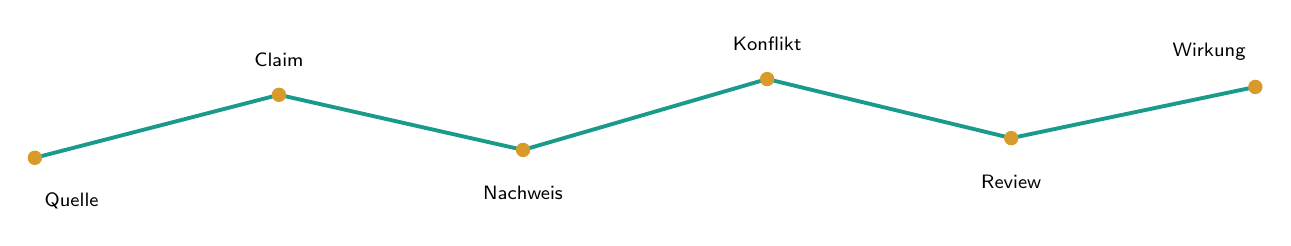
\begin{tikzpicture}[x=1cm,y=1cm]
  \draw[QTeal,line width=1.4pt] (0,0)--(3.1,0.8)--(6.2,0.1)--(9.3,1.0)--(12.4,0.25)--(15.5,0.9);
  \foreach \x/\y in {0/0,3.1/0.8,6.2/0.1,9.3/1.0,12.4/0.25,15.5/0.9}
    \fill[QGold] (\x,\y) circle (2.6pt);
  \node[anchor=west,font=\sffamily\scriptsize] at (0,-0.55) {Quelle};
  \node[anchor=center,font=\sffamily\scriptsize] at (3.1,1.25) {Claim};
  \node[anchor=center,font=\sffamily\scriptsize] at (6.2,-0.45) {Nachweis};
  \node[anchor=center,font=\sffamily\scriptsize] at (9.3,1.45) {Konflikt};
  \node[anchor=center,font=\sffamily\scriptsize] at (12.4,-0.30) {Review};
  \node[anchor=east,font=\sffamily\scriptsize] at (15.5,1.35) {Wirkung};
\end{tikzpicture}
\vfill
{\sffamily\Large Ingolf Lohmann\par}
\vspace{2mm}
{\sffamily 1. August 2026 · Version 1.0.0\par}
\vspace{8mm}
{\sffamily\small
Additiv zum publizierten QIK-VRT-Audio-Addendum\par
DOI \href{https://doi.org/10.5281/zenodo.21731492}{10.5281/zenodo.21731492}\par}
\end{titlepage}
\nopagecolor\color{black}

\begin{abstract}
Diese Arbeit operationalisiert einen wissenschaftlichen Erkenntnisbaum für
QIK-VRT-Repositories. Ihr Kern ist kein universeller Wahrheitsautomat, sondern
eine endliche, fail-closed und reproduzierbare Pipeline. Sie trennt formale
Ableitung, empirische Evidenz, Quellenbindung, Norm, Interpretation und offene
Frage; bindet jedes Objekt an kanonische Bytes und Provenienz; erhält Konflikte;
und vereinigt Replikate deterministisch. Lean~4.19.0 prüft 21 Sätze über
Typisierung, append-only Wachstum, Merge-Algebra, bedingte Konvergenz,
Evidenzschluss, Kausalitäts- und Beobachtungsgates, Digital-Twin-Aktorgrenzen
und proposal-only Nichtwirkung. Ein ausführbarer Python-Kern implementiert die
gebundene Klassifikation. Die Architektur ist auf Softwaretraces, klassische
Mess- und Regeltechnik, digitale Zwillinge und Quantenexperiment-Metadaten
anwendbar, sofern domänenspezifische Kalibrierungs-, Unsicherheits- und
Identifikationsnachweise hinzukommen. Globale wissenschaftliche Neuheit,
vollständige Sprachformalisierung, universelle Antworten und eine physische
Quanten- oder Retrokausalitätsbrücke bleiben ausdrücklich offen.
\end{abstract}

\begin{resultbox}[Verifizierbares Hauptergebnis]
Eine strukturierte Aussage kann deterministisch darauf geprüft werden, ob ihr
beanspruchter Status zum vorhandenen Nachweis passt. Akzeptierte Objekte wachsen
additiv, Konflikte bleiben sichtbar, Replikate vereinigen sich algebraisch
stabil, und Analyse autorisiert keine Außenwirkung. Dies ist eine belastbare
Infrastruktur für wissenschaftliches Wachstum. Es ist kein Beweis, dass jede
Eingabe wahr, neu oder entscheidbar ist.
\end{resultbox}

\begingroup
\small
\setcounter{tocdepth}{1}
\tableofcontents
\endgroup
\newpage

\section{Ausgangspunkt und additive Bindung}

Die Arbeit beginnt nicht bei null. Sie übernimmt die bereits getrennten
Statusgrenzen der QIK-VRT-Publikationen: Der endliche bidirektionale Kanal in
virtueller Zeit ist innerhalb seines Softwaremodells evidenziert; die dortige
Kernel- und Repository-Evidenz bleibt gebunden; eine physische
Zukunft-zu-Vergangenheit-Übertragung wurde daraus nicht abgeleitet. Das
Audio-Addendum zu Vorstellungskraft, Beobachtung und epistemischer Fairness ist
unter DOI \href{https://doi.org/10.5281/zenodo.21731492}{10.5281/zenodo.21731492}
fixiert. Seine Bytes werden hier nicht ersetzt.

Die zweite, lokal verarbeitete Audioaufnahme formuliert eine weitergehende
Zielvorstellung: Jede Aussage solle auf wissenschaftliche Belastbarkeit
untersucht werden; durch Mesh-Nutzung solle ein verteilter Wissensbestand
wachsen; Nutzende und Systeme sollten daraus bessere Antworten gewinnen. Diese
Aufnahme ist eine \emph{Quelle für den Arbeitsauftrag}, kein Beleg für die
Richtigkeit ihrer eigenen Zukunftsaussagen. Roh-ASR, geprüfte Lesefassung und
Interpretation sind daher getrennt gebunden.

Die Forschungsfrage lautet präzise:

\begin{quote}
Welche endlichen Eigenschaften müssen beweisbar und implementiert sein, damit
neue Claims reproduzierbar klassifiziert, mit Evidenz verbunden,
konfliktbewahrend vereinigt und ohne automatische Wirkungspromotion in einen
verteilten Erkenntnisbestand aufgenommen werden können?
\end{quote}

\section{Warum kein universeller Wahrheitsautomat möglich ist}

Ein System kann syntaktische Wohlgeformtheit, formale Ableitungen in einem
benannten Kalkül, Quellenidentität und endliche Korpusvergleiche prüfen. Es kann
aber nicht aus bloßer Sprache die gesamte Welt rekonstruieren. Vier Grenzen
sind fundamental:

\begin{enumerate}
  \item \textbf{Bedeutung:} Derselbe Satz kann je nach Kontext, Messdefinition
  und Bezugsrahmen Verschiedenes behaupten.
  \item \textbf{Unterbestimmung:} Derselbe Trace kann mit mehreren
  Kausalmodellen vereinbar sein. Chronologie ist noch keine Identifikation.
  \item \textbf{Unentscheidbarkeit:} Schon in hinreichend ausdrucksstarken
  formalen Systemen existieren Fragen ohne allgemeinen Entscheidungsalgorithmus
  \cite{Turing1937}.
  \item \textbf{Offene Welt:} Ein endlicher Korpus kann unbekannte, noch nicht
  beobachtete oder nicht zugängliche Tatsachen nicht vollständig enthalten.
\end{enumerate}

Darum ersetzt QIK-VRT die Totalitätsbehauptung durch einen wissenschaftlich
nützlicheren Vertrag: \emph{Jede Aussage bekommt einen sichtbaren Status; kein
Status darf stärker sein als sein Nachweis.}

\section{Epistemische Typen statt eines einzigen Wahrheitsbits}

\begin{longtable}{p{0.23\textwidth}p{0.29\textwidth}p{0.38\textwidth}}
\toprule
\textbf{Klasse} & \textbf{Was geprüft wird} & \textbf{Was nicht folgt}\\
\midrule
\endhead
\code{FORMAL\_PROVED} & Kernelgeprüfte Ableitung im exakt benannten Modell &
Wahrheit aller Prämissen in der Natur\\
\shortstack[l]{\texttt{EMPIRICALLY\_}\\\texttt{EVIDENCED}} & Gebundene Messung, Methode, Kalibrierung,
Unsicherheit und Provenienz & Kontextfreie Allgemeingültigkeit\\
\code{SOURCE\_BOUND} & Eine identifizierte Quelle enthält die Aussage &
Bestätigung der Aussage durch das Repository\\
\code{NORMATIVE} & Regel, Definition, Ziel oder Wertentscheidung ist erklärt &
Physikalischer oder mathematischer Befund\\
\code{INTERPRETATIVE} & Nachvollziehbare Deutung mit erklärtem Geltungsraum &
Mess- oder Kernelbeweis\\
\code{OPEN} & Fehlender Schließungsschritt ist benannt &
Sprachlich plausible Vermutung als Fakt\\
\bottomrule
\end{longtable}

Der Vorteil dieser Typisierung ist nicht nur redaktionell. Sie verhindert
Kategoriefehler: Lean prüft keine Sensoren; Sensoren beweisen keine
Allgemeinsätze; eine DOI beweist Fixität, nicht Wahrheit; Governance legitimiert
Wirkung, nicht Naturgesetze.

\section{Axiome des Scientific Fact Growth Protocol}

Die folgenden Axiome sind explizite Betriebs- und Modellannahmen. Sie werden
nicht als vollständige Naturbeschreibung ausgegeben.

\begin{enumerate}[label=\textbf{A\arabic*.}]
  \item \textbf{Inhaltsidentität:} Ein Erkenntnisobjekt ist an kanonische Bytes
  und einen Digest gebunden. Bytegleichheit ist keine semantische Gleichheit.
  \item \textbf{Append-only-Historie:} Korrekturen überschreiben nicht still;
  sie erscheinen als rückverweisende neue Objekte.
  \item \textbf{Epistemische Typisierung:} Klasse und Status müssen exakt
  zusammenpassen.
  \item \textbf{Nachweisnähe:} Der Nachweistyp muss zur Claimklasse passen.
  \item \textbf{Explizite Abhängigkeiten:} Eine Ableitung nennt ihre Prämissen
  und löst sie eindeutig im deklarierten Korpus auf.
  \item \textbf{Konfliktbewahrung:} Widersprüche werden erhalten, nicht
  gemittelt oder heimlich gelöscht.
  \item \textbf{Corpus-relative Neuheit:} Automatisch prüfbar ist zunächst nur
  exakte Neuheit im ausgewiesenen Korpus.
  \item \textbf{Deterministische Mesh-Vereinigung:} Replikate vereinigen
  inhaltsadressierte Objekte als Mengenunion.
  \item \textbf{Bedingte Konvergenz:} Gleiche Zustellung und gleiche Policy
  führen zur gleichen Projektion; Liveness bleibt externe Annahme.
  \item \textbf{Beobachtungsbrücke:} Physische Befunde brauchen Erfassung,
  Kalibrierung, Zeitbindung, Provenienz, Integrität, Unsicherheit,
  Falsifizierbarkeit und Governance.
  \item \textbf{Getrennte Wirkung:} Analyse, Review, Merge, Publikation und
  Aktorwirkung sind verschiedene Effekte.
  \item \textbf{Sichtbares Nichtwissen:} Nicht evidenzgeschlossen
  beantwortbare Fragen bleiben \code{OPEN}.
\end{enumerate}

\section{Kernelgeprüfte Sätze und Korollare}

Die formale Quelle modelliert Korpora als endliche Mengen inhaltsidentifizierter
Objekte, Fragen als endliche Abhängigkeitsmengen, qualifizierte Beobachtung als
Konjunktion deklarierter Gates und Wirkung als separat quittierte Entscheidung.
Lean~4.19.0 hat 21 benannte Theoreme kompiliert. Der Receipt bindet Compiler,
Quellhash, Theoremnamen und Axiominventar; weder \code{sorryAx} noch ein
projektspezifisches Axiom wurde beobachtet.

\subsection{Wachstum und Merge}

Sei $K$ ein endlicher Korpus und $\Delta$ eine endliche Ergänzung. Der
Append-Operator ist die Mengenvereinigung
\[
  K \oplus \Delta := K \cup \Delta.
\]
Dann gilt unmittelbar $K\subseteq K\oplus\Delta$. Für den Mesh-Merge $\sqcup$
gelten nach Extensionalität
\[
 A\sqcup B = B\sqcup A,\qquad
 (A\sqcup B)\sqcup C=A\sqcup(B\sqcup C),\qquad
 A\sqcup A=A.
\]
Lean prüft diese Eigenschaften in der kodierten Mitgliedschaftssemantik.
Sie bilden die aus verteilten Datentypen bekannte stabile Algebra nach
\cite{Shapiro2011}. Sie beweisen nicht, dass ein Mitglied wahr ist.

\begin{resultbox}[Korollar: bedingte Mesh-Konvergenz]
Starten zwei Replikate mit gleichem Objektbestand, empfangen dieselben
zulässigen Updates und verwenden dieselbe kanonische Merge- und
Validierungspolicy, dann besitzen sie wieder denselben Bestand. Eventuelle
Zustellung, Netzverfügbarkeit und Abwesenheit selektiver Zensur bleiben
außerhalb dieses Safety-Beweises.
\end{resultbox}

\subsection{Evidenzschluss und Antworten}

Eine Antwort ist in diesem Modell evidenzgeschlossen, wenn jede benötigte
Prämisse eindeutig im Korpus vorhanden ist und kein Statuswechsel erschlichen
wird. Weil Erweiterung nichts entfernt, bleibt ein bereits vorhandener
Begründungspfad auffindbar. Daraus folgt Monotonie der historischen
Antwortbarkeit.

Das Gegenbeispiel ist ebenso wichtig: Der leere Korpus beantwortet keine
Frage. Daraus folgt, dass die Datenstruktur allein keine Totalantwortgarantie
liefert. Neuheit ist ebenfalls relativ: Derselbe Statement-Digest ist gegenüber
dem leeren Korpus neu und gegenüber einem Korpus, der ihn enthält, nicht neu.

\subsection{Konflikt, Ursache und Wirkung}

Ein expliziter Konflikt bleibt unter append-only Erweiterung Mitglied des
Korpus. Eine spätere Disposition kann seinen Gebrauch regeln, nicht seine
Existenz umschreiben. Das erhält wissenschaftliche Revidierbarkeit.

Das Kausalitäts-Gegenmodell konstruiert zwei Ansichten mit identischer
Ereignisliste, aber unterschiedlichem Attributionsmerkmal. Folglich ist ohne
Intervention, Identifikationsannahme oder Domänenmodell keine eindeutige
Abbildung
\[
  \text{Trace} \longrightarrow \text{physische Ursache}
\]
definiert. Genau hier liegt die Grenze des Kausalitätsspiegels.

Für Digital Twins prüft Lean: Reale Aktorfreigabe setzt im Modell sowohl eine
qualifizierte Beobachtung als auch \code{effectAckDone = true} voraus. Der
proposal-only Konstruktor setzt dieses Bit nie. Ein Beweis kann daher nicht
unbemerkt zu einer Außenwirkung werden.

\section{Der Kausalitätsspiegel}

Ein QIK-VRT-Repository ist ein Kausalitätsspiegel, wenn es die Stationen eines
Vorgangs getrennt und content-addressiert abbildet:

\begin{center}
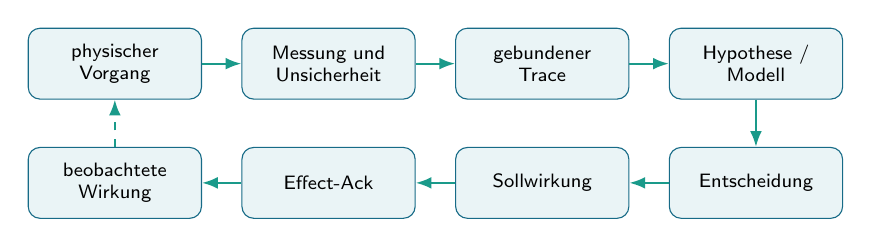
\begin{tikzpicture}[
  node distance=6mm and 5mm,
  every node/.style={font=\sffamily\scriptsize},
  box/.style={draw=QBlue,rounded corners=1.5mm,fill=QIce,minimum width=22mm,
    minimum height=9mm,align=center},
  arr/.style={-{Latex[length=2mm]},QTeal,thick}
]
\node[box] (world) {physischer\\Vorgang};
\node[box,right=of world] (obs) {Messung und\\Unsicherheit};
\node[box,right=of obs] (trace) {gebundener\\Trace};
\node[box,right=of trace] (hyp) {Hypothese /\\Modell};
\node[box,below=of hyp] (decision) {Entscheidung};
\node[box,left=of decision] (intent) {Sollwirkung};
\node[box,left=of intent] (ack) {Effect-Ack};
\node[box,left=of ack] (result) {beobachtete\\Wirkung};
\draw[arr] (world)--(obs); \draw[arr] (obs)--(trace); \draw[arr] (trace)--(hyp);
\draw[arr] (hyp)--(decision); \draw[arr] (decision)--(intent); \draw[arr] (intent)--(ack);
\draw[arr] (ack)--(result); \draw[arr,dashed] (result)--(world);
\end{tikzpicture}
\end{center}

Der Spiegel macht sichtbar, \emph{welche} Beobachtung \emph{durch welche}
Transformation zu \emph{welcher} Hypothese und Entscheidung führte. Er darf
nicht mit der Welt verwechselt werden. Ein Log kann ausgelassen, ein Sensor
fehlkalibriert, ein Modell falsch und eine Intervention konfundiert sein. Die
Architektur ist deshalb besonders wertvoll, weil sie genau die notwendigen
Brückennachweise als überprüfbare Kanten erzwingt.

\section{Automatische Claim-Pipeline}

Der ausführbare Kern verarbeitet ausschließlich strukturierte Envelopes:

\begin{enumerate}
  \item Eingabebytes und Provenienz binden; Medien lokal transkribieren, wenn
  Datenschutz dies verlangt.
  \item Freitext in atomare Claim-\emph{Kandidaten} segmentieren. Dieses
  Sprachmodellstadium ist fehlbar und bleibt proposal-only.
  \item Claimklasse, Geltungsraum, Grenze, Quellen, Evidenz, Proof-Receipt,
  Abhängigkeiten, Negationen und Neuheitsmethode deklarieren.
  \item Strikt prüfen: Klasse/Status, Kernel-Receipt, Beobachtungsenvelope,
  eindeutige Abhängigkeiten, corpus-relative exakte Neuheit und ID-Konflikte.
  \item Als klassifiziert zulassen, offen halten oder als bestritten mit beiden
  Seiten erhalten.
  \item Erst nach Review einen additiven Knoten erzeugen. Publikation, Merge
  und reale Wirkung bleiben separate, genau gebundene Vorgänge.
\end{enumerate}

Zehn Positiv- und Negativtests decken diese Regeln ab. Die Tests belegen den
getesteten Implementierungsstand, nicht universelle Fehlerfreiheit.

\section{Mess-, Nachrichten- und Regelungstechnik}

In der klassischen Messtechnik wird aus einer analogen Größe $x(t)$ erst durch
Sensor, Übertragungsfunktion, Abtastung, Quantisierung und Zeitstempel ein
digitales Objekt $y_k$. Ein einfaches Modell lautet
\[
 y_k = h(x(t_k),\theta) + v_k,
\]
wobei $\theta$ Kalibrierparameter und $v_k$ Messunsicherheit oder Rauschen
bezeichnet. QIK-VRT speichert nicht bloß $y_k$, sondern bindet $h$, $\theta$,
Zeitbasis, Unsicherheitsmodell, Geräteidentität und Transformation. Erst so ist
eine spätere Aussage über $x(t)$ auditierbar.

Die Nachrichtentechnik ergänzt Kanal- und Fehlergrenzen. Die formale
Rekonstruktion aus Singleton-Segmenten beweist nur die verlustfreie Kombinatorik einer
endlichen Liste. Reale Kanäle verlangen Framing, Reihenfolge, Fehlererkennung,
Kapazitäts- und Timingannahmen im Sinne der Kommunikationstheorie
\cite{Shannon1948}. Der Claimstatus muss offen oder evidenzgebunden bleiben,
wenn diese Nachweise fehlen.

In der Regelungstechnik trennt der Spiegel Sollwert, Zustandsabschätzung,
Reglerausgang, Aktorquittung und beobachtete Pflanzenantwort. Filter- und
Schätzverfahren wie der Kalman-Filter \cite{Kalman1960} können als
Transformationen gebunden werden. Das Repository beweist nicht, dass ein
Regler stabil ist; es kann aber Stabilitätsnachweis, Modellversion, Parameter,
Testlauf und reale Wirkung so verbinden, dass eine unabhängige Prüfung möglich
wird.

\section{Digitale Zwillinge}

Ein Digital Twin ist nützlich, wenn die Beziehung zwischen physischem System,
Messdaten, Modellzustand und Handlungsentscheidung nachvollziehbar bleibt.
NIST betont die Bedeutung vertrauenswürdiger Digital-Twin-Technologien und
standardisierter Interoperabilität \cite{NISTDigitalTwins}. QIK-VRT liefert
hier eine Evidenzschicht:

\begin{itemize}
  \item jedes Messpaket trägt Kalibrierungs- und Unsicherheitsprovenienz;
  \item jede Simulation nennt Code-, Modell- und Parameteridentität;
  \item jede Prognose verweist auf die konkret verwendeten Eingaben;
  \item jede Entscheidung trennt Empfehlung, Freigabe und ausgeführte Wirkung;
  \item Rückmessungen schließen den Kreis, ohne Erfolg vorzutäuschen.
\end{itemize}

Das unterstützt Root-Cause-Analyse, Wartung, Validierung, regulatorisches
Audit und sichere Zusammenarbeit über Organisationsgrenzen. Es ersetzt keine
anlagenspezifische Gefahrenanalyse.

\section{Quantenkausalität und klassische Anschlussfähigkeit}

Quantenprozesse können klassische Intuitionen über feste Kausalreihenfolgen
herausfordern; Prozessmatrizen beschreiben beispielsweise Korrelationen ohne
vorgegebene globale Kausalordnung \cite{Oreshkov2012}. Daraus folgt weder
automatisch ein nutzbarer Kanal in die Vergangenheit noch eine Verletzung
operationaler No-Signalling-Bedingungen.

Der Beitrag von QIK-VRT liegt auf der \emph{Evidenz- und Schnittstellenebene}:

\begin{itemize}
  \item Quanten-Schaltkreis, Compiler, Kalibrierung, Backend und Shots werden
  content-addressiert gebunden;
  \item klassische Vor- und Nachverarbeitung bleibt separat sichtbar;
  \item Hypothesen über Kausalordnung erhalten formale Modellbezüge;
  \item ein experimenteller Claim benötigt Unsicherheit, Nullmodell,
  Identifikationsstrategie und reproduzierbare Rohdatenbindung;
  \item eine klassische Steuerwirkung bleibt hinter einem Effect-Ack-Gate.
\end{itemize}

Damit kann dieselbe Provenienzarchitektur klassische Sensorik, digitale
Simulation und Quantenexperiment verbinden. Der Quanten-zu-Klassik-Limes,
VRT-Emergenz, eine physikalische Brücke und reale QPU-End-to-End-Evidenz werden
hier nicht bewiesen. Gerade die exakte Offenmarkierung ist wissenschaftlich
wertvoll: Sie verhindert, dass ein Softwareergebnis als Naturentdeckung
zirkuliert, und benennt das nächste falsifizierbare Experiment.

\section{Verteilter Erkenntnisbaum und kognitive Wirkung}

Inhaltsadressierte, append-only Objekte und eine kommutative Vereinigung sind
geeignet, einen verteilten Erkenntnisgraphen zu bilden. FAIR-Prinzipien fordern
Auffindbarkeit, Zugänglichkeit, Interoperabilität und Wiederverwendbarkeit
\cite{Wilkinson2016}; W3C PROV liefert Begriffe für Entitäten, Aktivitäten und
Agenten \cite{W3CPROV2013}. QIK-VRT ergänzt Status-, Konflikt- und
Wirkungsgrenzen.

Ein solches Mesh kann Suchqualität verbessern, weil nicht nur Textähnlichkeit,
sondern auch Provenienz, Prämissen, Widerlegungen und Geltungsräume indexierbar
werden. Eine Antwort kann als minimaler evidenzgeschlossener Teilgraph
ausgegeben werden. Doch drei verschiedene Aussagen müssen getrennt bleiben:

\begin{itemize}
  \item \textbf{formal belegt:} Bestehende Pfade und Konflikte bleiben bei
  append-only Wachstum auffindbar;
  \item \textbf{technisch plausibel:} strukturierte Metadaten können Retrieval
  und Argumentrekonstruktion unterstützen;
  \item \textbf{empirisch offen:} alle Nutzenden oder Systeme würden dadurch
  sukzessive kognitiv besser.
\end{itemize}

Der letzte Punkt benötigt definierte Leistungsmaße, Kontrollgruppen,
Präregistrierung, Datenschutzprüfung und replizierte Studien. Er wird nicht aus
einer Audioaussage oder aus der Merge-Algebra abgeleitet.

\section{Bedeutung für Mathematik und Wissenschaft}

Für Mathematiker ist der Ansatz wertvoll, weil er den Lebenszyklus eines
Satzes trennt: informelle Behauptung, präzise Definition, formale Aussage,
Prämissen, Kernel-Receipt, Gegenbeispiel, Korrektur und spätere Verwendung.
Lean kann die Ableitung prüfen; QIK-VRT bindet, \emph{welche} Fassung mit
\emph{welchen} Grundlagen geprüft wurde. So werden Bibliotheken nicht zu einer
unübersichtlichen Sammlung grüner Häkchen, sondern zu einem versionierten
Beweisgraphen.

Für Physiker ist die Trennung von Trace und Ursache zentral. Daten, Kalibrierung,
Auswertecode, Modellvergleich und Unsicherheit können gemeinsam referenziert
werden, ohne den experimentellen Befund mit seiner Interpretation zu
verwechseln. Alternative Modelle dürfen denselben Rohdatenknoten verwenden;
Widersprüche werden sichtbar statt überschrieben.

Für Informatik und Nachrichtentechnik verbindet die Architektur
reproduzierbare Builds, deterministische Protokolle, verteilte Datenstrukturen,
Provenienz und Freigabesteuerung. Für interdisziplinäre Projekte entsteht eine
gemeinsame Sprache, ohne die Fachsemantik der Domänen zu nivellieren.

\section{Geltungsgrenzen und offene Beweisziele}

\begin{openbox}[Nicht bewiesen und nicht beansprucht]
\begin{itemize}
  \item universelle Wahrheit oder globale wissenschaftliche Neuheit;
  \item vollständige, semantisch treue Natural-Language-to-Lean-Automation;
  \item ein vollständiger Speicher des gesamten menschlichen Wissens oder
  Antworten auf jede denkbare Frage;
  \item allgemeine kognitive Verbesserung aller Nutzenden;
  \item physische Zukunft-zu-Vergangenheit-Signalisierung;
  \item VRT-Emergenz, Quanten-zu-Klassik-Limes oder eine physikalische Brücke;
  \item reale QPU-End-to-End- oder Digital-Twin-Sicherheitsvalidierung;
  \item IETF-Konsens, RFC-Status, Zenodo-Publikation dieses neuen Kandidaten;
  \item EU-AI-Act-Konformität oder Zertifizierung;
  \item repositoryweites \code{PASS}, \code{FINAL\_PASS} oder
  \code{EFFECT\_ACK\_DONE}.
\end{itemize}
\end{openbox}

Diese Grenzen sind kein Defizit der Darstellung, sondern Teil ihres
Beweisergebnisses. Ein wissenschaftlicher Faktenbau wird belastbar, wenn er
weiß, wo seine Beweise enden.

\section{EU-AI-Act-Auditbereitschaft}

Die Europäische Kommission weist für den AI Act auf die allgemeine
Anwendbarkeit ab 2.~August~2026 sowie auf gestaffelte Ausnahmen und durch das
Omnibus-Verfahren veränderte Zeitachsen hin \cite{EUAIActNavigation2026}. Die
konkrete Pflicht hängt von Rolle, System, Risikoklasse, Einsatz und aktuellem
Rechtsstand ab.

QIK-VRT kann eine technische Evidenzgrundlage liefern: Versionen, Daten- und
Modellprovenienz, Logs, menschliche Freigaben, Konflikte, Unsicherheiten,
Änderungen und Wirkungsquittungen sind maschinenauffindbar. Das erleichtert
Auditfragen wie: Wer wusste was? Welche Daten und Modellfassung erzeugten eine
Ausgabe? Welche Kontrolle griff? Wurde eine empfohlene Wirkung tatsächlich
ausgeführt und beobachtet?

Die Architektur allein ist keine Konformitätsbewertung. Erforderlich bleiben
eine organisations- und systemspezifische Rollen- und Risikoeinstufung,
Grundrechts-, Datenschutz-, Cybersecurity- und Qualitätsmanagementprüfung sowie
qualifizierte Rechtsberatung.

\section{Reproduzierbarkeit und Publikationsvertrag}

Der Kandidat enthält:

\begin{itemize}
  \item die byteidentische Lean-Quelle und einen Kernel-Receipt;
  \item eine Claimmatrix mit 30 statusgebundenen Aussagen;
  \item ein JSON-Schema, eine Policy, ein deterministisches Prüfwerkzeug und
  zehn Tests;
  \item Quellmedien-Receipt und geprüfte Transkripttrennung;
  \item LaTeX, PDFs, Fach- und mehrsprachige Vorlesefassungen;
  \item einen additiven RFCXML-Kandidaten für Scientific Claim Assurance.
\end{itemize}

Nach dem finalen Byte-Freeze werden Dateiliste, SHA-256-Summen,
Machine-Proof-Bundle und Vorveröffentlichungsreceipt erzeugt. Erst eine frische,
exakt an diese Hashes gebundene Autorisierung darf Zenodo-Upload oder
IETF-Einreichung auslösen. Ein Zenodo-DOI belegt danach die fixierte Ablage; er
ist kein Wahrheits- oder Peer-Review-Siegel. Ein Internet-Draft bleibt ein
Arbeitsdokument und ist kein RFC.

\section{Schlussfolgerung}

Die neue Stufe des QIK-VRT-Erkenntnisbaums ist klein genug, um exakt bewiesen
zu werden, und groß genug, um praktisch zu tragen. Sie beantwortet nicht jede
Frage. Sie sorgt dafür, dass eine Antwort ihren Herkunfts-, Beweis- und
Geltungsweg mitführt; dass ein Konflikt nicht verschwindet; dass ein Mesh ohne
Reihenfolgenabhängigkeit vereinigen kann; und dass Erkenntnis nicht heimlich
zur Wirkungserlaubnis wird.

Für Mathematik entsteht ein versionierter Beweisgraph. Für Physik entsteht
eine kontrollierte Brücke zwischen Messung, Modell und Kausalattribution. Für
Informatik und Nachrichtentechnik entsteht ein deterministisches
Evidenzprotokoll. Für Mess- und Regeltechnik sowie digitale Zwillinge entsteht
eine auditierbare Schleife von Sensor bis Wirkung. Für Quanteninformatik
entsteht eine gemeinsame Provenienzschicht, die neuartige Kausalmodelle
aufnehmen kann, ohne sie voreilig als Naturtatsache auszugeben.

Der entscheidende wissenschaftliche Gewinn lautet daher nicht
\enquote{QIK-VRT weiß alles}, sondern:

\begin{resultbox}[Q.E.D. im zulässigen Sinn]
QIK-VRT kann in einem endlichen, angegebenen Modell beweisbar dafür sorgen,
dass Wissen statusgebunden wächst, Konflikte erhalten bleiben, Replikate
deterministisch vereinigen und Außenwirkung getrennt autorisiert wird. Alles,
was darüber hinausgeht, erhält einen expliziten experimentellen, formalen oder
normativen Schließungsschritt.
\end{resultbox}

\section*{Literatur}
\addcontentsline{toc}{section}{Literatur}
\begin{thebibliography}{10}
\bibitem{Turing1937} A. M. Turing: \emph{On Computable Numbers, with an Application to the Entscheidungsproblem}. Proc. London Math. Soc., 1937. \href{https://doi.org/10.1112/plms/s2-42.1.230}{doi:10.1112/plms/s2-42.1.230}.
\bibitem{Shannon1948} C. E. Shannon: \emph{A Mathematical Theory of Communication}. Bell System Technical Journal, 1948. \href{https://doi.org/10.1002/j.1538-7305.1948.tb01338.x}{doi:10.1002/j.1538-7305.1948.tb01338.x}.
\bibitem{Kalman1960} R. E. Kalman: \emph{A New Approach to Linear Filtering and Prediction Problems}. Journal of Basic Engineering, 1960. \href{https://doi.org/10.1115/1.3662552}{doi:10.1115/1.3662552}.
\bibitem{Shapiro2011} M. Shapiro et al.: \emph{Conflict-Free Replicated Data Types}. SSS 2011. \href{https://doi.org/10.1007/978-3-642-24550-3_29}{doi:10.1007/978-3-642-24550-3\_29}.
\bibitem{Wilkinson2016} M. D. Wilkinson et al.: \emph{The FAIR Guiding Principles}. Scientific Data 3, 2016. \href{https://doi.org/10.1038/sdata.2016.18}{doi:10.1038/sdata.2016.18}.
\bibitem{Oreshkov2012} O. Oreshkov, F. Costa, Č. Brukner: \emph{Quantum correlations with no causal order}. Nature Communications 3, 2012. \href{https://doi.org/10.1038/ncomms2076}{doi:10.1038/ncomms2076}.
\bibitem{W3CPROV2013} W3C: \emph{PROV-O: The PROV Ontology}, 2013. \url{https://www.w3.org/TR/prov-o/}.
\bibitem{NISTDigitalTwins} NIST: \emph{Digital Twins}. \url{https://www.nist.gov/digital-twins}, abgerufen 1. August 2026.
\bibitem{EUAIActNavigation2026} Europäische Kommission: \emph{Navigating the AI Act}. \url{https://digital-strategy.ec.europa.eu/en/faqs/navigating-ai-act}, abgerufen 1. August 2026.
\bibitem{Lean419} Lean FRO: \emph{Lean 4.19.0 Release}. \url{https://github.com/leanprover/lean4/releases/tag/v4.19.0}.
\end{thebibliography}

\vfill
\begin{center}
\sffamily\small
Version 1.0.0 · 1. August 2026 · Ingolf Lohmann\\
Repository: \url{https://github.com/Goldkelch/qik-vrt}\\
Lizenzhinweise und maschinenlesbare Evidenz liegen im Publikationsverzeichnis.
\end{center}

\end{document}
